\documentclass[11pt]{article}
\usepackage[margin=1in]{geometry}
\usepackage[pdftex]{graphicx}
\usepackage{amsmath,amssymb,amsthm}
\usepackage{custom}

% plotting
\usepackage{pgfplots}
\pgfplotsset{compat=1.18}

% color boxes
\usepackage[many]{tcolorbox}
\tcbuselibrary{theorems}
\newtcbtheorem{psexample}{Example}{colback=green!10,colframe=green!40!black,fonttitle=\bfseries,breakable,enhanced}{ex}
\newtcbtheorem{psidea}{Idea}{colback=blue!10,colframe=blue!40!black,fonttitle=\bfseries,breakable,enhanced}{id}
\newtcbtheorem{psremark}{Remark}{colback=purple!10,colframe=purple!40!black,fonttitle=\bfseries,breakable,enhanced}{rm}
\newtcbtheorem{pssolution}{Solution}{colback=orange!10,colframe=orange!40!black,fonttitle=\bfseries,breakable,enhanced}{sn}
\tcbset{noparskip/.style={before={\par\pagebreak[0]\medskip\parindent=0pt},
after={\par\medskip}}}

% code for totaling up points
\usepackage{totcount}
\newtotcounter{tpts}
\newtotcounter{cpts}
\newtotcounter{endpts}
\newcommand{\clearpts}{\addtocounter{tpts}{\value{cpts}} \setcounter{cpts}{0}}
\newcommand{\pts}[1]{\clearpts \setcounter{cpts}{#1}}
\newcommand{\totpts}{\setcounter{endpts}{\totvalue{tpts} + \totvalue{cpts}}\arabic{endpts}}

% formatting for problems and solutions
\definecolor{ptred}{rgb}{0.7,0.1,0.1}
\newcommand{\ptfmt}[1]{\textbf{\color{ptred}#1\color{black}}}
\definecolor{advblue}{rgb}{0.1,0.1,0.7}
\newcommand{\advanced}{\!\textbf{\color{advblue}[A]\color{black}}\ }

\newtheorem*{solution}{Solution}
\newtheorem*{answer}{Answer}

\makeatletter
\newtheoremstyle{mystyle}
{\topsep}               % space above
{\topsep}               % space below
{}                      % bodyfont
{}                      % indent
{\bfseries}             % headfont
{}                      % punctuation
{0.6em}                 % space after head
{\llap{[\ptfmt{\arabic{cpts}}]\hspace{.6em}}\thmname{#1}\thmnumber{ #2}\thmnote{\normalfont{ (#3)}}{\bfseries .}}  %theoremheadspec
\theoremstyle{mystyle}
\newtheorem{pproblem}{Problem}
\makeatother

% clocks for time limits
\usepackage{clock}
\ClockFrametrue\ClockStyle=1

% headers and footers
\usepackage{fancyhdr}
\pagestyle{fancy}
\lhead{Taylor Series}
\chead{}
\rhead{F = ma Toolkit}
\lfoot{}
\cfoot{\thepage}
\rfoot{}
\renewcommand{\headrulewidth}{0.4pt}
\setlength{\headheight}{14pt}

\newcommand{\psettitle}[1]{
    \begin{center}
    \huge \textbf{#1}
    \end{center}
}

\linespread{1.03} % give a little extra room
\setlength{\parindent}{0.2in} % reduce paragraph indent a bit

% ============================================================
% SOLUTIONS TOGGLE
% Set \showsoltrue to PRINT solutions, \showsolfalse to HIDE them.
% (When building from the command line you can instead pass
%  \def\HIDESOLUTIONS{} to force the student/no-solutions version.)
% ============================================================
\newif\ifshowsol
\showsoltrue                       % <-- flip to \showsolfalse for the student copy
\ifdefined\HIDESOLUTIONS \showsolfalse \fi

\usepackage{environ}
\ifshowsol\else
  \NewEnviron{killsol}{}
  \let\solution\killsol
  \let\endsolution\endkillsol
  \let\answer\killsol
  \let\endanswer\endkillsol
\fi

\begin{document}

\psettitle{Taylor Series for the F = ma Exam}
\begin{center}
\large A fluency-first toolkit: a handful of approximations you will use everywhere
\end{center}

\noindent
This handout is not about \emph{proving} anything. You do not need calculus, and you do
not need to know what ``convergence'' means. The goal is fluency: by the end you should
be able to look at $e^{0.03}$, $\sqrt{1.02}$, $\cos(0.1)$, or $1/\sqrt{1-v^2/c^2}$ and
write down a good estimate in one line. These five facts and their uses appear over and
over in introductory physics and on the F = ma exam. There is a total of
\ptfmt{\totpts} points. Problems marked \advanced are a little harder.

\section{The One Idea}

\begin{psidea}{Near a point, every curve looks simple}{}
Zoom in on any smooth curve and it starts to look like a straight line; zoom out a
little and it looks like a parabola. A \textbf{Taylor series} is just a recipe for
writing a complicated function as
\[
\text{(a constant)} \;+\; \text{(something)}\times x \;+\;
\text{(something)}\times x^2 \;+\; \cdots
\]
where $x$ is measured from the point you zoomed in on. When $x$ is \emph{small}, the
later terms shrink fast and you can throw them away. That is the whole game.
\end{psidea}

\begin{psidea}{``Small'' means high powers are negligible}{}
If $x = 0.1$, then $x^2 = 0.01$ and $x^3 = 0.001$. Each power is ten times smaller than
the last. So if you only care about $1\%$ accuracy, keeping the $x$ term and dropping
$x^2$ is completely safe. The smaller $x$ is, the fewer terms you need. We write
$\approx$ (``approximately equals'') to mean ``equal once we drop the tiny leftover
terms.''
\end{psidea}

\pts{3}
\begin{pproblem}
Let $x = 0.02$. Compute $x$, $x^2$, and $x^3$. If you want an answer good to about
$0.1\%$ (one part in a thousand), which of these terms can you safely ignore?
\end{pproblem}
\begin{solution}
$x = 0.02$, $x^2 = 0.0004$, $x^3 = 0.000008$. One part in a thousand is $0.001$. The
$x^2 = 0.0004$ term is right at the edge and might matter; $x^3 = 8\times10^{-6}$ is far
below $0.001$ and is completely safe to drop. So you would keep through $x^2$ and ignore
$x^3$ and beyond.
\end{solution}

\section{The Five You Must Memorize}

\begin{psidea}{The whole toolkit on one line each}{}
For \textbf{small} $x$ (and angles in \textbf{radians}):
\[
\boxed{\,(1+x)^n \approx 1 + nx\,}\qquad
\boxed{\,e^{x} \approx 1 + x\,}\qquad
\boxed{\,\ln(1+x) \approx x\,}
\]
\[
\boxed{\,\sin x \approx x\,}\qquad\qquad
\boxed{\,\cos x \approx 1 - \tfrac{1}{2}x^2\,}
\]
That is the entire handout in five boxes. Everything below is either a reason these are
true, a graph of how good they are, or a place in physics where they save you. Notice
sine keeps only \emph{one} term (its next term is tiny, $-x^3/6$), while the others keep
\emph{two}.
\end{psidea}

\begin{psremark*}{}{}
Two cautions. (1) These hold only when $x$ is small compared to $1$. ``$x$ small'' for
$\sin x \approx x$ literally means the angle in \emph{radians} is small --- $\sin(30^\circ)$
is \emph{not} close to $30$. (2) In $(1+x)^n$ the small quantity is $x$, not the whole
base; you often have to massage a number into the form $1 + (\text{small})$ first.
\end{psremark*}

\begin{psexample}{One-line estimates}{}
\[
e^{0.05} \approx 1 + 0.05 = 1.05 \quad(\text{true: } 1.0513),\qquad
\cos(0.1) \approx 1 - \tfrac12(0.1)^2 = 0.995 \quad(\text{true: } 0.99500).
\]
\end{psexample}

\pts{5}
\begin{pproblem}
Estimate each in one line using the boxed formulas, without a calculator:
\begin{subpart}
\item $e^{0.01}$
\item $\sin(0.02)$
\item $\cos(0.2)$
\item $(1.03)^{4}$ \quad (here $x = 0.03$, $n = 4$)
\item $\ln(1.04)$
\end{subpart}
\end{pproblem}
\begin{solution}
(a) $e^{0.01}\approx 1+0.01 = 1.01$.\quad
(b) $\sin(0.02)\approx 0.02$.\quad
(c) $\cos(0.2)\approx 1-\tfrac12(0.2)^2 = 1-0.02 = 0.98$.\quad
(d) $(1.03)^4 \approx 1 + 4(0.03) = 1.12$ (true $1.1255$).\quad
(e) $\ln(1.04)\approx 0.04$.
\end{solution}

\section{More Terms, Better Fit}

\begin{psidea}{Each new term widens the range where the fit is good}{}
The full series for our functions are
\[
e^x = 1 + x + \tfrac{x^2}{2} + \tfrac{x^3}{6} + \cdots,\qquad
\cos x = 1 - \tfrac{x^2}{2} + \tfrac{x^4}{24} - \cdots,\qquad
\sin x = x - \tfrac{x^3}{6} + \tfrac{x^5}{120} - \cdots
\]
You almost never need past the first two terms, because we only ever use these when $x$
is small. But it is worth \emph{seeing} what the extra terms buy you: one term matches
the curve at a point, two terms match it over a small neighborhood, three terms over a
wider one. The plots below show the true function (thick) against the 1-, 2-, and
3-term approximations.
\end{psidea}

\begin{center}
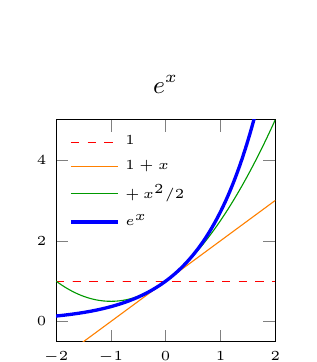
\begin{tikzpicture}
\begin{axis}[
  title={$e^x$}, title style={font=\small},
  width=0.36\textwidth, height=4.4cm,
  domain=-2:2, samples=80,
  xmin=-2, xmax=2, ymin=-0.5, ymax=5,
  tick label style={font=\tiny}, label style={font=\tiny},
  legend style={font=\tiny, at={(0.02,0.98)}, anchor=north west, draw=none, fill=none},
  legend cell align=left,
]
\addplot[red, dashed]   {1};                 \addlegendentry{$1$}
\addplot[orange]        {1+x};               \addlegendentry{$1+x$}
\addplot[green!60!black]{1+x+x^2/2};         \addlegendentry{$+\,x^2/2$}
\addplot[blue, very thick] {exp(x)};         \addlegendentry{$e^x$}
\end{axis}
\end{tikzpicture}
\hfill
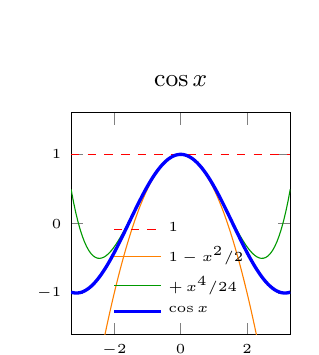
\begin{tikzpicture}
\begin{axis}[
  title={$\cos x$}, title style={font=\small},
  width=0.36\textwidth, height=4.4cm,
  domain=-3.3:3.3, samples=100,
  xmin=-3.3, xmax=3.3, ymin=-1.6, ymax=1.6,
  tick label style={font=\tiny}, label style={font=\tiny},
  legend style={font=\tiny, at={(0.5,0.03)}, anchor=south, draw=none, fill=none},
  legend cell align=left,
]
\addplot[red, dashed]    {1};                       \addlegendentry{$1$}
\addplot[orange]         {1-x^2/2};                  \addlegendentry{$1-x^2/2$}
\addplot[green!60!black]  {1-x^2/2+x^4/24};          \addlegendentry{$+\,x^4/24$}
\addplot[blue, very thick]{cos(deg(x))};            \addlegendentry{$\cos x$}
\end{axis}
\end{tikzpicture}
\hfill
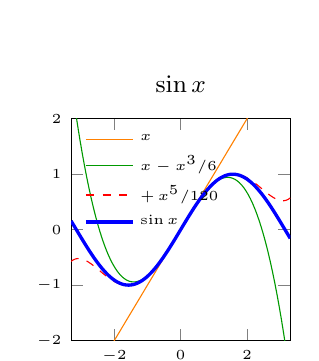
\begin{tikzpicture}
\begin{axis}[
  title={$\sin x$}, title style={font=\small},
  width=0.36\textwidth, height=4.4cm,
  domain=-3.3:3.3, samples=100,
  xmin=-3.3, xmax=3.3, ymin=-2, ymax=2,
  tick label style={font=\tiny}, label style={font=\tiny},
  legend style={font=\tiny, at={(0.02,0.98)}, anchor=north west, draw=none, fill=none},
  legend cell align=left,
]
\addplot[orange]          {x};                       \addlegendentry{$x$}
\addplot[green!60!black]  {x-x^3/6};                  \addlegendentry{$x-x^3/6$}
\addplot[red, dashed]     {x-x^3/6+x^5/120};          \addlegendentry{$+\,x^5/120$}
\addplot[blue, very thick]{sin(deg(x))};             \addlegendentry{$\sin x$}
\end{axis}
\end{tikzpicture}
\end{center}

\begin{psremark*}{}{}
Look at $\sin x \approx x$ near the middle of its plot: the straight line $y = x$ hugs
the true sine curve all the way out to about $x = 0.5$ before peeling away. That is why
the small-angle approximation is so good for pendulums --- the swing angles are small.
\end{psremark*}

\pts{4}
\begin{pproblem}
Using the cosine series $\cos x \approx 1 - \tfrac{x^2}{2} + \tfrac{x^4}{24}$, estimate
$\cos(1)$ (that is one radian, about $57^\circ$) keeping (a) one term, (b) two terms,
(c) three terms. The true value is $0.5403$. Watch the estimate march toward it.
\end{pproblem}
\begin{solution}
(a) $1$. \quad
(b) $1 - \tfrac12 = 0.5$. \quad
(c) $1 - 0.5 + \tfrac{1}{24} = 0.5417$. \quad
Each term gets dramatically closer to $0.5403$: the one-term answer is useless here
because $x=1$ is not small, but by three terms we are good to better than $0.3\%$.
\end{solution}

\section{Powers and Roots: $(1+x)^n \approx 1 + nx$ for \emph{any} $n$}

\begin{psidea}{$n$ can be anything --- negative, a fraction, whatever}{}
The single formula $(1+x)^n \approx 1 + nx$ does not care what $n$ is. Three favorites:
\[
\frac{1}{1+x} = (1+x)^{-1} \approx 1 - x,\qquad
\sqrt{1+x} = (1+x)^{1/2} \approx 1 + \tfrac{x}{2},\qquad
\frac{1}{\sqrt{1+x}} = (1+x)^{-1/2} \approx 1 - \tfrac{x}{2}.
\]
A square root is nothing special: it is just the power $n = \tfrac12$. Since
$(1+x)^n \approx 1 + nx$, we get $\sqrt{1+x} \approx 1 + \tfrac12 x$ for free.
\end{psidea}

\begin{psexample}{Estimating $\sqrt{65}$ by hand}{}
$\sqrt{65}$ looks hard, but $65 = 64\,(1 + \tfrac{1}{64})$, and $\sqrt{64} = 8$ is easy.
So
\[
\sqrt{65} = 8\,\sqrt{1 + \tfrac{1}{64}} \approx 8\left(1 + \tfrac12\cdot\tfrac{1}{64}\right)
         = 8\left(1 + \tfrac{1}{128}\right) = 8 + \tfrac{8}{128} = 8.0625.
\]
The true value is $8.0623$. We got four correct digits with mental arithmetic. The trick
is always the same: \textbf{pull out the nearest easy value} so what is left is
$1 + (\text{small})$.
\end{psexample}

\begin{psexample}{Why $\tfrac12 mv^2$ is the low-speed limit of relativity}{}
You may have met Einstein's $E = mc^2$. The fuller statement of special relativity is
that a mass $m$ moving at speed $v$ has total energy $E = \gamma\, mc^2$, where the
\textbf{gamma factor} is
\[
\gamma = \frac{1}{\sqrt{1 - v^2/c^2}} = \left(1 - \tfrac{v^2}{c^2}\right)^{-1/2},
\]
and $c$ is the speed of light. We will just take this as a given fact. The number
$\gamma$ is always at least $1$; at everyday speeds $v \ll c$ it is barely above $1$, and
it grows large only as $v$ approaches $c$. The energy of motion (kinetic energy) is the
part beyond the rest energy $mc^2$, namely $(\gamma - 1)mc^2$. Now Taylor-expand: with
$x = -v^2/c^2$ small,
\[
\gamma \approx 1 - \tfrac12\!\left(-\tfrac{v^2}{c^2}\right) = 1 + \tfrac12\frac{v^2}{c^2},
\]
so the kinetic energy $(\gamma - 1)mc^2 \approx \tfrac12 m v^2$. The familiar
$\tfrac12 mv^2$ you already know is just the first Taylor term of the exact relativistic
energy.
\end{psexample}

\pts{6}
\begin{pproblem}
Estimate each by pulling out the nearest easy value, in one or two lines:
\begin{subpart}
\item $\sqrt{101}$ \quad (use $100\cdot(1+\tfrac{1}{100})$)
\item $\dfrac{1}{0.98}$
\item $(1.01)^{10}$
\item $\sqrt[3]{8.6}$ \quad (use $8\cdot(1+\tfrac{0.6}{8})$, $n = \tfrac13$)
\item $\dfrac{1}{\sqrt{1.04}}$
\item $\sqrt{0.96}$
\end{subpart}
\end{pproblem}
\begin{solution}
(a) $\sqrt{101} = 10\sqrt{1+0.01}\approx 10(1+0.005) = 10.05$ (true $10.0499$).\quad
(b) $\dfrac{1}{0.98} = (1-0.02)^{-1}\approx 1+0.02 = 1.02$ (true $1.0204$).\quad
(c) $(1.01)^{10}\approx 1+10(0.01) = 1.10$ (true $1.1046$).\quad
(d) $\sqrt[3]{8.6} = 2(1+0.075)^{1/3}\approx 2(1+0.025) = 2.05$ (true $2.0488$).\quad
(e) $(1.04)^{-1/2}\approx 1-0.02 = 0.98$ (true $0.9806$).\quad
(f) $\sqrt{0.96} = (1-0.04)^{1/2}\approx 1-0.02 = 0.98$ (true $0.9798$).
\end{solution}

\pts{3}
\begin{pproblem}
A pendulum's period is $T = 2\pi\sqrt{L/g}$. A clock's pendulum is lengthened by
$0.5\%$. By what percentage does its period change? (Use $\sqrt{1+x}\approx 1+\tfrac{x}{2}$.)
\end{pproblem}
\begin{solution}
$T \propto \sqrt{L}$, so $T \to T\sqrt{1+0.005}\approx T(1+0.0025)$: the period grows by
about $0.25\%$. (Half the fractional change in $L$, because of the square root.)
\end{solution}

\section{Logarithms: $\ln(1+x) \approx x$}

\begin{psidea}{Read it off from $e^x$}{}
The logarithm undoes the exponential: $\ln(e^x) = x$. Now use $e^x \approx 1 + x$. If we
call $u = e^x - 1 \approx x$, then $1 + u \approx e^x$, so
\[
\ln(1+u) \approx \ln(e^x) = x \approx u.
\]
In words: for small $u$, $\ln(1+u) \approx u$. The log of something just above $1$ is
about how far above $1$ it is.
\end{psidea}

\pts{4}
\begin{pproblem}
Estimate, one line each:
\begin{subpart}
\item $\ln(1.1)$
\item $\ln(0.97)$ \quad (write $0.97 = 1 + (-0.03)$)
\item $\ln(1.005)$
\item Sound level grows like $\ln$. If a sound's intensity rises by $2\%$, roughly how
much does $\ln(\text{intensity})$ increase?
\end{subpart}
\end{pproblem}
\begin{solution}
(a) $\ln(1.1)\approx 0.1$ (true $0.0953$).\quad
(b) $\ln(0.97)\approx -0.03$ (true $-0.0305$).\quad
(c) $\ln(1.005)\approx 0.005$.\quad
(d) $\ln(1.02)\approx 0.02$, an increase of about $0.02$.
\end{solution}

\section{Even and Odd Functions}

\begin{psidea}{Symmetry decides which powers can appear}{}
A function is \textbf{even} if $f(-x) = f(x)$ --- its graph is a mirror image across the
vertical axis. It is \textbf{odd} if $f(-x) = -f(x)$ --- its graph looks the same after
a $180^\circ$ rotation about the origin. Powers are the simplest examples:
\[
x^0,\ x^2,\ x^4,\ \dots \text{ are even};\qquad x^1,\ x^3,\ x^5,\ \dots \text{ are odd}.
\]
This forces the shape of a Taylor series:
\begin{itemize}
\item An \textbf{even} function's series uses \emph{only even powers}. That is why
$\cos x = 1 - \tfrac{x^2}{2} + \tfrac{x^4}{24} - \cdots$ has no $x$, no $x^3$.
\item An \textbf{odd} function's series uses \emph{only odd powers}. That is why
$\sin x = x - \tfrac{x^3}{6} + \cdots$ has no constant, no $x^2$.
\end{itemize}
Cosine is even, sine is odd. You can use this as a memory check: if you ever ``derive''
a $\cos x \approx 1 + ax$ with a stray linear term, you know it is wrong, because cosine
is even.
\end{psidea}

\pts{4}
\begin{pproblem}
Classify each as even, odd, or neither: (a) $x^2 + \cos x$, \;(b) $x\,\cos x$,
\;(c) $\sin x + x^3$, \;(d) $e^x$.
\end{pproblem}
\begin{solution}
(a) even (sum of two even things). \quad
(b) odd (odd $\times$ even $=$ odd). \quad
(c) odd (sum of two odd things). \quad
(d) neither --- its series $1 + x + \tfrac{x^2}{2}+\cdots$ mixes even and odd powers.
\end{solution}

\pts{3}
\begin{pproblem}
A potential energy $U(x)$ near $x = 0$ is known to be an \emph{even} function (the system
looks the same if you flip $x \to -x$). Explain why its expansion must look like
$U(x) \approx U_0 + \tfrac12 k\,x^2$ with no term linear in $x$ --- and why that means a
mass placed there feels a spring-like (harmonic) force.
\end{pproblem}
\begin{solution}
Even functions contain only even powers, so the $x^1$ term is forbidden; the first thing
after the constant $U_0$ is an $x^2$ term, which we name $\tfrac12 k x^2$. A potential of
the form $U_0 + \tfrac12 k x^2$ is exactly that of a spring, so the motion is harmonic.
The symmetry alone guarantees no linear term, which is what kills any constant
(non-restoring) force at the center.
\end{solution}

\section{Physics Applications}

\begin{psidea}{Small-angle pendulum}{}
For a pendulum of length $L$ swinging through angle $\theta$, the restoring force along
the arc is proportional to $\sin\theta$. Using $\sin\theta \approx \theta$,
\[
\text{restoring force} \propto \sin\theta \approx \theta,
\]
which is the defining feature of simple harmonic motion (force proportional to
displacement). That single approximation is why a pendulum keeps near-constant time and
why $T = 2\pi\sqrt{L/g}$ is independent of amplitude --- \emph{as long as the swing is
small}. In energy language, the height gives
$U = mgL(1-\cos\theta) \approx mgL\cdot\tfrac12\theta^2 = \tfrac12(mgL)\theta^2$,
a perfect parabola in $\theta$: a spring with effective stiffness $mgL$.
\end{psidea}

\begin{psidea}{Every potential is a spring near its minimum}{}
This is the most important application on the whole list. Take \emph{any} potential
energy $U(x)$ with a minimum at $x = x_0$. Expand in the small displacement
$\delta = x - x_0$:
\[
U(x) \approx U(x_0) + (\text{slope at } x_0)\,\delta + \tfrac12 k\,\delta^2 + \cdots
\]
At a minimum the slope is zero, so the linear term \emph{vanishes}. The first term that
survives is the $\delta^2$ term:
\[
\boxed{\,U(x) \approx U(x_0) + \tfrac12 k\,\delta^2\,}
\]
which is a spring. So a mass near \emph{any} potential minimum oscillates harmonically
with $\omega = \sqrt{k/m}$, where $k$ is whatever number multiplies $\tfrac12\delta^2$.
Molecules, atoms in a crystal, a ball in a bowl, a pendulum --- all of them are springs
when you look closely enough at the bottom.
\end{psidea}

\begin{psexample}{Lennard--Jones: a molecule is a spring}{}
Two atoms interact with the Lennard--Jones potential
$U(r) = 4\varepsilon\!\left[(\sigma/r)^{12} - (\sigma/r)^{6}\right]$, which has a minimum
at some spacing $r_0$. Near $r_0$ the linear term is absent (it is a minimum), so
$U(r) \approx U(r_0) + \tfrac12 k(r-r_0)^2$. The molecule therefore vibrates like a tiny
mass on a spring of stiffness $k$ --- exactly the model used for molecular vibration
frequencies. The complicated $r^{-12}$ and $r^{-6}$ powers are irrelevant once you are
close to the bottom; only the curvature $k$ matters.
\end{psexample}

\begin{psidea}{Gravity a little above the surface}{}
Newton's law gives $g(h) = \dfrac{GM}{(R+h)^2}$ at height $h$ above a planet of radius
$R$. Factor out $R$:
\[
g(h) = \frac{GM}{R^2}\frac{1}{(1+h/R)^2} = g_0\,(1 + h/R)^{-2} \approx g_0\!\left(1 - \frac{2h}{R}\right).
\]
So gravity weakens roughly \emph{linearly} with height near the surface, losing a
fraction $2h/R$ of its strength. (The factor of $2$ comes straight from $n = -2$.)
\end{psidea}

\begin{psidea}{Radioactive decay over a short time}{}
A sample decays as $N(t) = N_0\,e^{-\lambda t}$. For times short compared with the
lifetime ($\lambda t \ll 1$), use $e^{-\lambda t} \approx 1 - \lambda t$:
\[
N(t) \approx N_0(1 - \lambda t),
\]
so the fraction that has decayed is about $\lambda t = t/\tau$, growing linearly at
first. This is why ``activity'' (decays per second) is nearly constant over short
windows even though the true law is exponential.
\end{psidea}

\pts{3}
\begin{pproblem}
At what height $h$ (as a fraction of Earth's radius $R \approx 6400$ km) does gravity drop
by $1\%$? Use $g(h) \approx g_0(1 - 2h/R)$.
\end{pproblem}
\begin{solution}
Set $2h/R = 0.01$, so $h/R = 0.005$ and $h \approx 0.005 \times 6400\text{ km} = 32$ km.
A $1\%$ drop in $g$ takes only about $32$ km of altitude.
\end{solution}

\pts{3}
\begin{pproblem}
A radioactive source has lifetime $\tau = 1/\lambda = 10$ hours. Using
$e^{-\lambda t}\approx 1 - \lambda t$, estimate the fraction that has decayed after
(a) $6$ minutes and (b) $30$ minutes. Why would this approximation be terrible for
estimating the fraction left after $40$ hours?
\end{pproblem}
\begin{solution}
$\lambda = 1/(10\text{ h})$. (a) $t = 0.1$ h, fraction decayed $\approx \lambda t = 0.01$,
i.e.\ $1\%$. (b) $t = 0.5$ h, fraction $\approx 0.05$, i.e.\ $5\%$. After $40$ h,
$\lambda t = 4$, which is not small at all --- $1 - \lambda t = -3$ is nonsense (you
cannot have a negative amount). The linear approximation only works while $\lambda t \ll 1$.
\end{solution}

\pts{4}
\begin{pproblem}
Show that the pendulum potential $U(\theta) = mgL(1 - \cos\theta)$ reduces to a spring
for small swings, and identify the effective spring constant in the variable $\theta$.
Then argue in one sentence why the period does not depend on the amplitude of a small
swing.
\end{pproblem}
\begin{solution}
Using $\cos\theta \approx 1 - \tfrac12\theta^2$, we get
$U \approx mgL\bigl(1 - (1 - \tfrac12\theta^2)\bigr) = \tfrac12(mgL)\theta^2$, a spring
with ``stiffness'' $mgL$ in $\theta$. Because the restoring effect is exactly
proportional to the displacement $\theta$ (no higher powers survive), the oscillation
frequency is set by the stiffness and inertia alone, not by how far you pull it back ---
so the period is amplitude-independent for small swings.
\end{solution}

\section{Propagation of Error}

\begin{psidea}{A power multiplies your percentage error by $n$}{}
Suppose you measure a quantity with a small fractional (percentage) error $\epsilon$, so
your value is really $A(1+\epsilon)$. If a result depends on it as a power, $Q = A^n$, then
\[
Q = A^n(1+\epsilon)^n \approx A^n(1 + n\epsilon).
\]
The fractional error in $Q$ is about $n\epsilon$: \textbf{powers scale percentage errors
by the exponent}. Squaring doubles your error; a square root halves it; an inverse-square
($n = -2$) doubles it (the sign just says the error goes the other way).
\end{psidea}

\begin{psexample}{From a pendulum's period to $g$}{}
You time a pendulum to get $g$ from $T = 2\pi\sqrt{L/g}$, i.e.\ $g \propto T^{-2}$. Here
$n = -2$, so a $1\%$ error in your measured period $T$ becomes a
$|{-2}|\times 1\% = 2\%$ error in $g$. Timing matters twice as much as you might guess.
\end{psexample}

\pts{3}
\begin{pproblem}
You measure the radius of a sphere to $1\%$. What is the resulting percentage error in
(a) its surface area $\propto r^2$ and (b) its volume $\propto r^3$?
\end{pproblem}
\begin{solution}
(a) $n = 2$: error $\approx 2 \times 1\% = 2\%$.\quad
(b) $n = 3$: error $\approx 3 \times 1\% = 3\%$. Higher powers amplify the measurement
error in proportion to the exponent.
\end{solution}

\pts{3}
\begin{pproblem}
Kinetic energy is $K = \tfrac12 m v^2$. If a speed is known to $2\%$, to what percentage
is the kinetic energy known (assume $m$ is exact)? If instead you want $K$ good to $1\%$,
how precisely must you know $v$?
\end{pproblem}
\begin{solution}
$K \propto v^2$, so $n = 2$ and the error is $\approx 2 \times 2\% = 4\%$. To get $K$ to
$1\%$ you need $v$ to $0.5\%$ (since $2\times 0.5\% = 1\%$).
\end{solution}

\pts{4}
\begin{pproblem} \advanced
A quantity is built as $Q = \dfrac{a\,b^2}{\sqrt{c}}$, where $a$, $b$, $c$ are measured
with small fractional errors $\epsilon_a$, $\epsilon_b$, $\epsilon_c$. Using
$(1+\epsilon)^n \approx 1 + n\epsilon$ on each factor, show that the fractional error in
$Q$ is approximately $\epsilon_a + 2\epsilon_b + \tfrac12\epsilon_c$ in the worst case,
and explain where each coefficient comes from.
\end{pproblem}
\begin{solution}
Write each measured value as its true value times $(1+\epsilon)$. Then
\[
Q \propto a^{1} b^{2} c^{-1/2}
\;\to\; (1+\epsilon_a)^1(1+\epsilon_b)^2(1+\epsilon_c)^{-1/2}
\approx (1+\epsilon_a)(1+2\epsilon_b)(1-\tfrac12\epsilon_c).
\]
Multiplying out and keeping only first-order terms (products of two small $\epsilon$'s
are negligible) gives $1 + \epsilon_a + 2\epsilon_b - \tfrac12\epsilon_c$. So the
fractional error coefficients are exactly the exponents: $1$ for $a$, $2$ for $b$ (it is
squared), and $\tfrac12$ for $c$ (it is under a square root). In the worst case the errors
add in size, giving $\epsilon_a + 2\epsilon_b + \tfrac12\epsilon_c$.
\end{solution}

\vspace{1em}
\begin{center}
\emph{End of handout. If you remember only the five boxes in Section 2 and the trick of
pulling out the nearest easy value, you already have what the F = ma exam asks of you.}
\end{center}

\end{document}
